\documentclass[12pt]{article}
\usepackage{fix-cm}

\usepackage[a4paper,
            top=3cm, bottom=2cm,
            left=3cm, right=2cm]{geometry}

\usepackage[num, overcite]{abntex2cite}
\citebrackets[]
\makeatletter
\renewcommand\@biblabel[1]{[#1] }
\makeatother

\usepackage{subcaption}
\usepackage{booktabs}
\usepackage{amsmath, amsfonts, amsthm, bm}
\usepackage{newtxtext, newtxmath, mathtools}
\usepackage[brazil]{babel}
\usepackage[T1]{fontenc}
\usepackage{indentfirst}
\usepackage{microtype}
\usepackage{fancyhdr}
\usepackage{graphicx}
\usepackage{ragged2e}
\usepackage{multirow}
\usepackage{setspace}
% subfig removido: é incompatível com subcaption, já carregado acima
\usepackage{icomma}
\usepackage{array}
\usepackage{float}
\usepackage{tikz}

\usepackage{silence}
\WarningFilter{latex}{Command \showhyphens has changed}

\onehalfspacing
\setlength{\parindent}{1.25cm}
\setlength{\parskip}{0.4\baselineskip}
\justifying

\usepackage{titlesec}

\newcommand{\titlefix}{
  \hyphenpenalty=10000
  \exhyphenpenalty=10000
  \emergencystretch=2em
}

\captionsetup{
    justification=centering
}

\titleformat{\section}
{\normalsize\bfseries\titlefix}
{\thesection.}
{0.5em}
{}

\titlespacing*{\section}
{0.75cm}
{1.5\baselineskip}
{0.8\baselineskip}

\titleformat{\subsection}
{\normalsize\bfseries\titlefix}
{\thesubsection.}
{0.5em}
{}

\titlespacing*{\subsection}
{1.5cm}
{1.2\baselineskip}
{0.6\baselineskip}

\titleformat{\subsubsection}
{\normalsize\bfseries\titlefix}
{\thesubsubsection.}
{0.5em}
{}

\titlespacing*{\subsubsection}
{2.25cm}
{1.0\baselineskip}
{0.4\baselineskip}

\titleformat{name=\section,numberless}
{\normalsize\bfseries\centering\titlefix}
{}
{0em}
{}

\titlespacing*{name=\section,numberless}
{0cm}
{1.5\baselineskip}
{0.8\baselineskip}

\usepackage{graphicx}
% imagens desta semana + logotipo herdado da semana 1
\graphicspath{{imagens_semana2/}{./}}
\usepackage{listings} 

\lstset{
  language=[LaTeX]TeX,
  basicstyle=\ttfamily\small, 
  breaklines=true,            
  frame=single,               
  keywordstyle=\color{blue}   
}

\begin{document}
\pagestyle{empty}

\begin{center}

	
\includegraphics[width=0.3\textwidth]{ita_rgb.jpg}

	\vfill

	{\large\bfseries
		Relatório parcial semanas 2 e 3\\[2.0\baselineskip]

	}

	\vfill

	{\normalsize\bfseries
		Caio Schaden Ishida\\[0.5\baselineskip]
		Cauã Henrique de Souza\\[0.5\baselineskip]
		Felipe Osternes da Silva\\[0.5\baselineskip]
		Henrique Sousa Fagundes\\[0.5\baselineskip]
		João Victor Evers Cordeiro\\[0.5\baselineskip]
		José Hernando Figueiredo da Silva Filho
	}

	\vfill

	{\normalsize\bfseries
		Grupo nº 07\\[0.6\baselineskip]
		Turma 30.2
	}

	\vfill

	{\normalsize
		Professores\\
		Deborah Dibbern Brunelli\\
		Leonardo Tsuyoshi Ueno\\
		Luís Gustavo Ferroni Pereira\\

		\medskip

		Data de entrega: 26/08/2026
	}

	\vfill

	{\normalsize\bfseries
		Departamento de Química\\
		Divisão de Ciências Fundamentais\\
		Instituto Tecnológico de Aeronáutica - ITA
	}

\end{center}


\newpage

\section{Atividades das semanas 2 e 3}

As principais metas das semanas 2 e 3 em relação ao desenvolvimento do \textit{software} foram cumpridas sem maiores complicações. O código desenvolvido em \textit{MATLAB} nas semanas anteriores foi concluído e aperfeiçoado e, a partir dele, o programa foi implementado como um aplicativo \textit{web}. Dessa forma, o usuário acessa a ferramenta por um endereço eletrônico, sem precisar instalar nenhum programa nem dispor de licença de \textit{software} pago, e todos os cálculos são realizados no próprio navegador.

A interface foi construída de modo que o usuário informe apenas o que pretende medir e quais condições consegue controlar no laboratório, com os respectivos valores mínimo e máximo, conforme mostra a Figura \ref{fig:entrada}. Com essas informações, o programa monta o planejamento composto central e apresenta os ensaios em ordem aleatória, indicando os valores de cada variável em cada ensaio.

\begin{figure}[H]
	\centering
	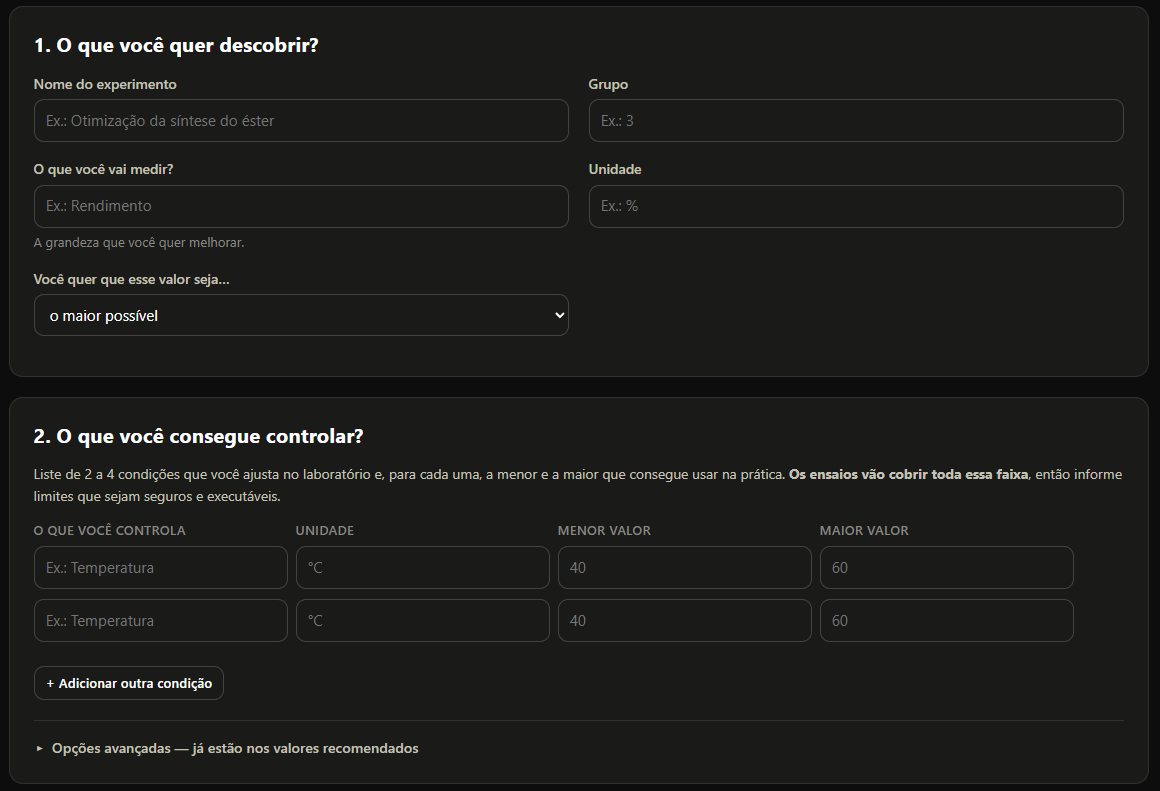
\includegraphics[width=0.72\linewidth]{figura1_melhor.png}
	\caption{Tela de entrada dos dados do experimento, preenchida antes da geração dos ensaios.}
	\label{fig:entrada}
\end{figure}

Dentro do software, após a geração dos 11 ensaios, estes são exportados em uma planilha do \textit{Excel} (Figura \ref{fig:planilha}), que traz uma coluna em branco destinada aos resultados. Assim, uma vez terminados os experimentos, o grupo preenche essa coluna e devolve o mesmo arquivo ao programa, que realiza o ajuste do modelo e a análise dos dados.

\begin{figure}[H]
	\centering
	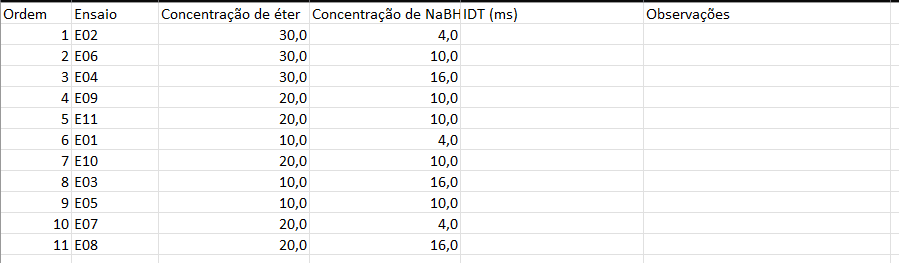
\includegraphics[width=0.88\linewidth]{figura_experimento_correto1.png}
	\caption{Planilha gerada pelo programa, com a coluna de resultado a ser preenchida em branco.}
	\label{fig:planilha}
\end{figure}

Concluída a análise, foi implementada uma funcionalidade no programa para retornar a condição ótima dentro da região estudada e o valor previsto para a resposta, acompanhados de uma avaliação da qualidade do ajuste, como mostra a Figura \ref{fig:resultado}. Dentro dessa avaliação, também são apresentados os gráficos dos resultados, entre eles o mapa da superfície de resposta da Figura \ref{fig:superficie}, no qual as cores representam o valor previsto em toda a região experimental e os ensaios realizados aparecem sobrepostos, com a condição ótima sendo destacada.

\begin{figure}[H]
	\centering
	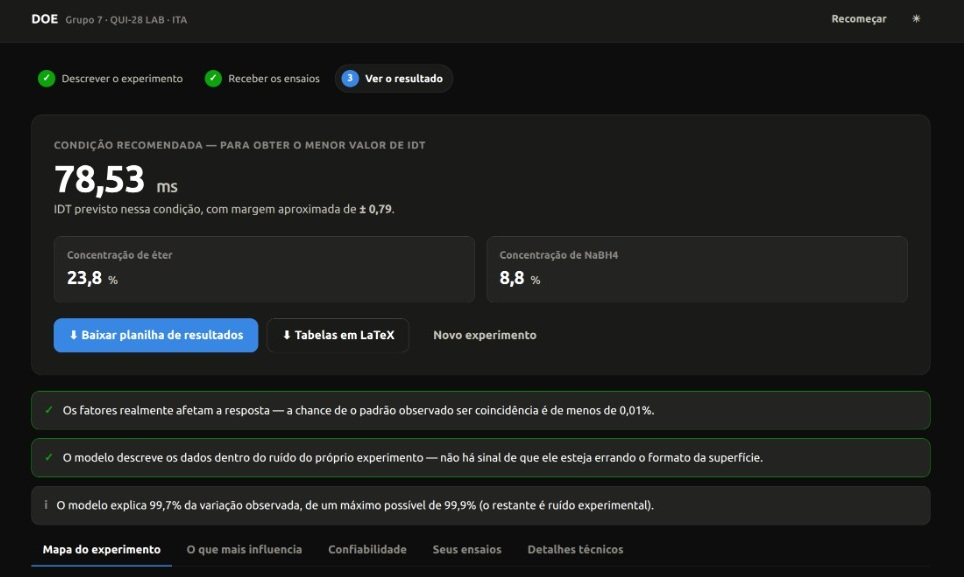
\includegraphics[width=0.86\linewidth]{img8_correta_atualizada.jpeg}
	\caption{Condição ótima e avaliação do ajuste retornadas pelo programa.}
	\label{fig:resultado}
\end{figure}

\begin{figure}[H]
	\centering
	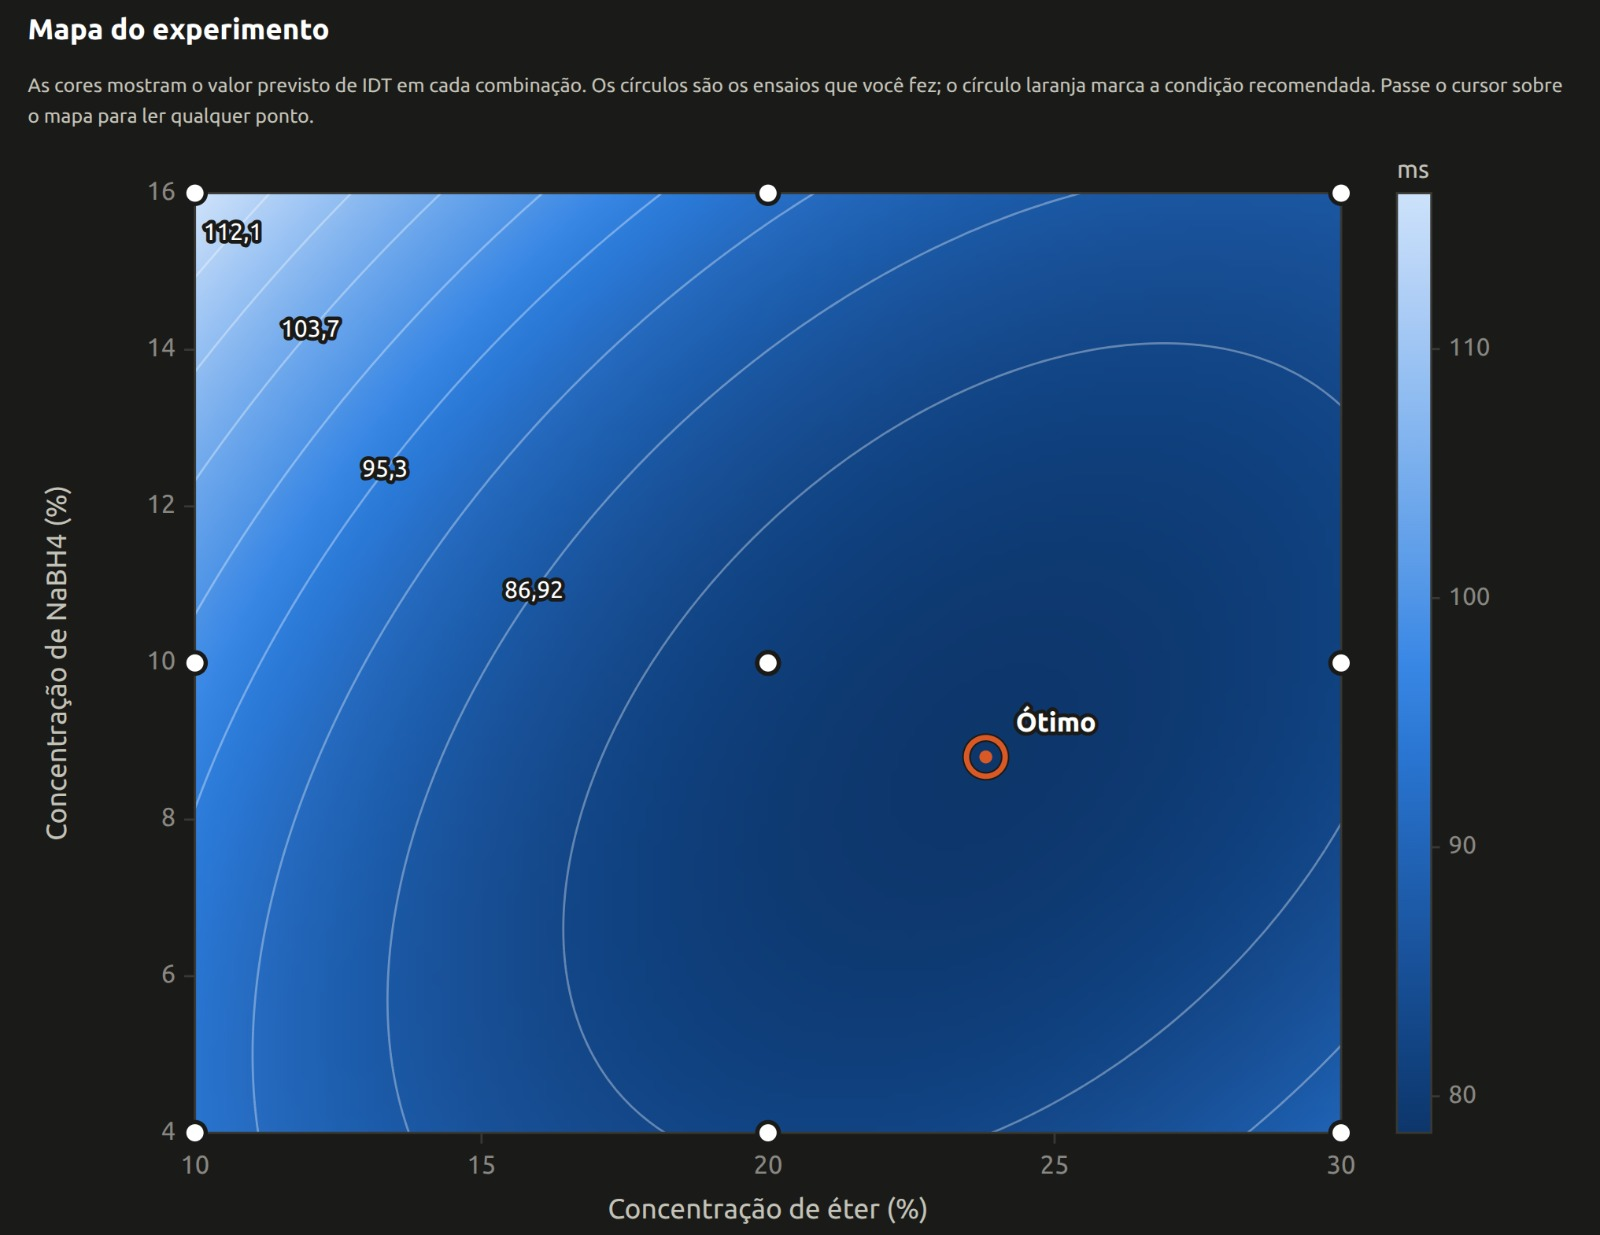
\includegraphics[width=0.52\linewidth]{img9.jpeg}
	\caption{Mapa da superfície de resposta.}
	\label{fig:superficie}
\end{figure}

Dentre as metas, foram cumpridas tarefas secundárias que irão auxiliar os experimentalistas na escrita dos seus relatórios. A lógica implementada em \textit{MATLAB}, que fornece automaticamente o código \textit{LaTeX} de uma tabela de dados e da análise de variância, foi concluída e, em seguida, tomada como base para a construção da versão final integrada ao aplicativo. Mantendo aquele mesmo formato, a exportação passou a ser feita diretamente pelo programa, que gera as tabelas já preenchidas e sem os campos de referência em branco que existiam na versão anterior. A Tabela \ref{tab:ANOVA} é exatamente a saída do programa para o experimento das figuras anteriores: os resultados são organizados e a tabela é gerada automaticamente ao final da análise, bastando inseri-la no relatório.

\begin{table}[H]
	\centering
	\caption{Análise de variância gerada automaticamente pelo programa.}
	\label{tab:ANOVA}

	\renewcommand{\arraystretch}{1.25}
	\begin{tabular}{l c c c c}
		\toprule
		\textbf{Fonte de variação}  & \textbf{Soma quadrática} & \textbf{Nº de g.l.} & \textbf{Média quadrática} & \textbf{$F$} \\
		\midrule
		Regressão                   & 1175,107                 & 5                   & 235,021                   & 365,30       \\
		Resíduos                    & 3,217                    & 5                   & 0,643                     &              \\
		\quad Falta de ajuste       & 1,752                    & 3                   & 0,584                     & 0,80         \\
		\quad Erro puro             & 1,465                    & 2                   & 0,732                     &              \\
		\midrule
		Total                       & 1178,324                 & 10                  & 117,832                   &              \\
		\midrule
		\% de variação explicada    & 99,73\%                  &                     &                           &              \\
		\bottomrule
	\end{tabular}
\end{table}

Diferentemente da primeira versão, feita em \textit{MATLAB}, a tabela passou a separar, dentro dos resíduos, a parcela devida ao erro do próprio experimento (erro puro) daquela devida à falta de ajuste do modelo, o que só é possível porque o planejamento gerado inclui repetições no ponto central.

Além disso, foi implementado um sistema de \textit{save state}, onde as informações fornecidas, como os dados das variáveis de otimização, são salvas e a etapa onde o usuário está também é salva, ou seja, se o programa for fechado e aberto novamente, ele não será resetado, mas voltará para a etapa em que estava antes de ser encerrado.

\section{Planejamento para as semanas 4 e 5}

Os principais objetivos para as semanas 4 e 5 envolvem o aperfeiçoamento do aplicativo \textit{web} desenvolvido, focando na revisão de suas funcionalidades e correção de eventuais \textit{bugs}. Para tanto, é necessário simular um projeto e testar cada uma das funcionalidades que o aplicativo oferece, como planejamento aleatório dos ensaios, tratamento estatístico dos dados, significância dos modelos gerados, obtenção do ponto ótimo, \textit{plot} de gráficos \textit{etc}. Os exemplos utilizados nos testes do aplicativo são apresentados por Bruns \textit{et al.}\cite{barrosneto2001}.

Cada funcionalidade será testada em pares, a fim de garantir a redundância na identificação das eventuais falhas do programa. Cada um dos pares de revisão irá documentar as propostas de alteração, discutir as principais prioridades e comunicá-las aos demais integrantes do grupo para o aperfeiçoamento do código.

A principal meta do período, no entanto, é a elaboração de um guia completo de utilização do \textit{software}, de modo que não restem dúvidas aos demais grupos sobre o processo de uso. Pretende-se também verificar o funcionamento do aplicativo sem acesso à internet, por meio de um servidor local em \textit{Python} ou da extensão \textit{Live Server} do \textit{VSCode}, e acompanhar os demais grupos durante as primeiras utilizações, cabendo a cada integrante o grupo que já assessora, de modo a garantir que todos consigam utilizá-lo sem dificuldades.

Quanto à interface, pretende-se melhorar as cores, acrescentar novas seções e esclarecer alguns pontos que hoje ficam implícitos. Um exemplo é a escolha da distribuição dos ensaios: as opções apresentadas descrevem apenas o efeito de cada configuração, sem indicar o valor de $\alpha$ correspondente, informação útil para quem for descrever o planejamento no relatório.

Ao mesmo tempo, pretende-se continuar documentando cada alteração e sua respectiva razão. Cada uma das funcionalidades será testada pelos pares de acordo com a Tabela \ref{tab:tarefas}.

\begin{table}[H]
	\centering
	\caption{Atribuição de tarefas para as semanas 4 e 5}
	\begin{tabular}{l p{8.4cm}}
		\toprule
		\textbf{Integrantes} & \textbf{Atividade}                                                                                                                          \\
		\midrule
		Caio Schaden                 & Revisar as demais atividades e documentar as alterações propostas                                                                    \\
		Cauã Souza                   & Verificar a geração do planejamento e a aleatorização da ordem dos ensaios                                                           \\
		Felipe Osternes              & Verificar a ida e volta das planilhas e a execução do aplicativo sem acesso à internet                                               \\
		João Evers e José Hernando   & Verificar o tratamento estatístico com diferentes conjuntos de resultados, conferindo se o modelo ajustado e o ponto ótimo correspondem ao esperado \\
		Henrique Fagundes            & Elaborar o guia de utilização e implementar as melhorias de interface                                                                \\
		\bottomrule
	\end{tabular}
	\label{tab:tarefas}
\end{table}

Por fim, depois do cumprimento desses objetivos, pretende-se implementar uma lógica que perfome um Teste F para avaliar a significância estatística de termos específicos no modelo obtido por meio da regressão linear.

\newpage

\section*{Referências bibliográficas}
\begingroup
\renewcommand{\section}[2]{}
\bibliography{referencias}
\endgroup

\end{document}
